scope
named parameters
methods on types

In the following example we declare a simple function which calculates
\gomarginpar{Some text in this chapter comes from \cite{go_intro}.}  % layout
the factorial value of a value \var{x}.

\begin{lstlisting}
func Factorial(x int) int {
   if x == 0 {
      return 1;	
   } else {
      return x * Factorial(x - 1);
   }
}
\end{lstlisting}

Go extends that by adding support for named return values. You can 
\gomarginindex{named return values}{named return values}
declare the return value as a variable in the function header; then you
can assign values to that variable. When the function returns, the last
value assigned to the return variable is the return value. So you could
also write factorial as:

\begin{lstlisting}
func Factorial(x int) (result int) {
  if x == 0 {
    result = 1;	
  } else {
    result = x * Factorial(x - 1);
  }
  return;
}
\end{lstlisting}
You can also write a function with multiple return values:

\begin{lstlisting}
func fib(n) (val int, pos int) {
   if n == 0 {
      val = 1;
      pos = 0;
   } else if n == 1 {
      val = 1;
      pos = 1;
   } else {
      v1, _ := fib(n-1);
      v2,_ := fib(n-2);
      val = v1 + v2;
      pos = n;
   }
   return;
}
\end{lstlisting}
(The above contained boneheaded mistake 1: I just wrote that out, and didn't bother to compile it. Naturally, I screwed it up in a silly way. It's since been fixed.)

defer, multiple return values etc etc

ection{Exercises}
\begin{Exercise}[title={Stack},difficulty=5]
\label{ex:stack}
\Question \label{ex:stack q1} Create a simple stack which can hold a
fixed amount of \key{int}s. Is does not have to grow beyond this limit.
Define both a \func{push} and \func{pop} function.

\begin{wrapfigure}{l}{30mm}
\begin{center}
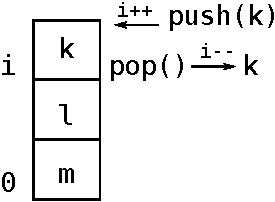
\includegraphics[scale=0.50]{fig/stack.pdf}
\end{center}
\end{wrapfigure}

\Question \label{ex:stack q2} Bonus. Write a \func{String} method which 
converts the stack to a string. This way you can print the stack using:
\lstinline{fmt.Printf("My stack %v\n", stack)}. This may aid in
debugging.
\end{Exercise}

\begin{Answer}

\Question 

\Question 

\end{Answer}


\cleardoublepage
\section{Answers}
\shipoutAnswer
